\documentclass[modern, letterpaper]{aastex62}

% to-do list
% ----------
% -

\include{gitstuff}
% Load common packages
% \usepackage{microtype}  % ALWAYS!
\usepackage{amsmath}
\usepackage{amsfonts}
\usepackage{amssymb}
\usepackage{booktabs}

\usepackage{graphicx}
\usepackage{color}

\definecolor{cbblue}{HTML}{3182bd}
\usepackage{hyperref}
\definecolor{linkcolor}{rgb}{0.02,0.35,0.55}
\definecolor{citecolor}{rgb}{0.45,0.45,0.45}
\hypersetup{colorlinks=true,linkcolor=linkcolor,citecolor=citecolor,
            filecolor=linkcolor,urlcolor=linkcolor}
\hypersetup{pageanchor=true}

\newcommand{\documentname}{\textsl{Article}}
\newcommand{\sectionname}{Section}
\renewcommand{\figurename}{Figure}
\newcommand{\eqname}{Equation}
\renewcommand{\tablename}{Table}

% Packages / projects / programming
\newcommand{\package}[1]{\textsl{#1}}
\newcommand{\acronym}[1]{{\small{#1}}}
\newcommand{\github}{\package{GitHub}}
\newcommand{\python}{\package{Python}}
\newcommand{\emcee}{\project{emcee}}

% Missions
\newcommand{\project}[1]{\textsl{#1}}

% For referee
\newcommand{\changes}[1]{{\color{red} #1}}

% Stats / probability
\newcommand{\given}{\,|\,}
\newcommand{\norm}{\mathcal{N}}

% Maths
\newcommand{\dd}{\mathrm{d}}
\newcommand{\transpose}[1]{{#1}^{\mathsf{T}}}
\newcommand{\inverse}[1]{{#1}^{-1}}
\newcommand{\argmin}{\operatornamewithlimits{argmin}}
\newcommand{\mean}[1]{\left< #1 \right>}

% Unit shortcuts
\newcommand{\msun}{\ensuremath{\mathrm{M}_\odot}}
\newcommand{\kms}{\ensuremath{\mathrm{km}~\mathrm{s}^{-1}}}
\newcommand{\mps}{\ensuremath{\mathrm{m}~\mathrm{s}^{-1}}}
\newcommand{\pc}{\ensuremath{\mathrm{pc}}}
\newcommand{\kpc}{\ensuremath{\mathrm{kpc}}}
\newcommand{\kmskpc}{\ensuremath{\mathrm{km}~\mathrm{s}^{-1}~\mathrm{kpc}^{-1}}}

% Misc.
\newcommand{\bs}[1]{\boldsymbol{#1}}
\definecolor{mahogany}{RGB}{165,15,21}
\newcommand{\resp}[1]{{\color{mahogany}#1}}

% Astronomy
\newcommand{\DM}{{\rm DM}}
\newcommand{\feh}{\ensuremath{{[{\rm Fe}/{\rm H}]}}}
\newcommand{\df}{\acronym{DF}}

% TO DO
\newcommand{\todo}[1]{{\color{red} TODO: #1}}


% adjust AAS-TEX shit
% \setlength{\parindent}{1.1\baselineskip}

\graphicspath{{figures/}}

% define macros for text
\newcommand{\apogee}{\project{\acronym{APOGEE}}}
\newcommand{\sdssiv}{\project{\acronym{SDSS-IV}}}
\newcommand{\thejoker}{\project{The~Joker}}
\newcommand{\thecannon}{\project{The~Cannon}}
\newcommand{\DR}{\acronym{DR14}}
\newcommand{\DRtw}{\acronym{DR12}}
\newcommand{\RC}{\acronym{RC}}
\newcommand{\RGB}{\acronym{RGB}}
\newcommand{\quantile}[2]{\ensuremath{\textrm{Q}_{#1}}\left(#2\right)}
\newcommand{\pdf}{\textit{pdf}}

\newcommand{\nstars}{96,231}
\newcommand{\nhighK}{4,510}
\newcommand{\nbimodal}{113}
\newcommand{\nunimodal}{319}

% for response to referee
% \renewcommand{\resp}[1]{#1}

\shortauthors{Price-Whelan et al.}

\begin{document}\sloppy\sloppypar\raggedbottom\frenchspacing % trust me

\title{Tidal circularization of companions to evolved stars}

\author[0000-0003-0872-7098]{Adrian~M.~Price-Whelan}
\affiliation{Department of Astrophysical Sciences,
             Princeton University, Princeton, NJ 08544, USA}
\email{adrn@astro.princeton.edu}
\correspondingauthor{Adrian M. Price-Whelan}

\author[0000-0003-2866-9403]{David~W.~Hogg}
\affiliation{Max-Planck-Institut f\"ur Astronomie,
             K\"onigstuhl 17, D-69117 Heidelberg, Germany}
\affiliation{Center for Cosmology and Particle Physics,
             Department of Physics,
             New York University, 726 Broadway,
             New York, NY 10003, USA}
\affiliation{Center for Data Science,
             New York University, 60 Fifth Ave,
             New York, NY 10011, USA}
\affiliation{Flatiron Institute,
             Simons Foundation,
             162 Fifth Avenue,
             New York, NY 10010, USA}

\author[0000-0003-4996-9069]{Hans-Walter~Rix}
\affiliation{Max-Planck-Institut f\"ur Astronomie,
             K\"onigstuhl 17, D-69117 Heidelberg, Germany}

\begin{abstract}\noindent % trust me
% Context
% Aims
% Methods
% Results
\end{abstract}

\keywords{
  binaries:~spectroscopic
}

\section{Introduction} \label{sec:intro}

From studies of binary star systems in open clusters, it is clear that
short-period binaries tend to be more circular (have smaller eccentricities) as
compared to longer-period binaries of the same age (e.g.,
\citealt{Mathieu:2005}).
Within a given population of binaries, this manifests as an apparently steep
transition from a distribution of eccentricities to mainly circularized orbits
at some characteristic period that depends on the age and evolutionary state of
the population (see, e.g., \figurename~5 in \citealt{Mathieu:2005})---i.e. above
this critical value of the period (or log-period), systems have some
distribution of eccentricities, and below the eccentricities are close to zero.
Many studies have measured this ``circularization period,'' predominantly for
main-sequence binaries (e.g., \citealt{Meibom:2006, Kjurkchieva:2017}), and
have found that it tends to be between 5--20 days, depending on age (e.g.,
\citealt{Mathieu:1988}).
For giant stars, the circularization period appears to be longer, closer to
$\approx 100$ days (\citealt{Mayor:1984}).

Theories for the tidal circularization process generally rely on tidal
dissipation via eddy viscosity in the convective regions of stars to explain
this (e.g., \citealt{Zahn:1989}).
The circularization timescale and period should therefore depend on the size of
the convective region, and the stellar parameters of the primary star.
RGB stars are therefore excellent test-cases for these theories, since
they are fully-convective:
By comparing to (small) samples of giant star binaries in open clusters, it
seems that the circularization timescales predicted by eddy viscosity
dissipation at least qualitatively scale to giant stars
(\citealt{Verbunt:1995}).

It is less clear what to expect for red clump (\RC) stars:
RC stars are horizontal branch stars and have therefore already climbed the RGB.
Short period, circularized companions in place before or while on the RGB could
be engulfed, or will at least have been common-envelope with the evolving star.
However, it is difficult to select samples of \RC\ stars to study this process
because first-ascent RGB stars will have similar colors and stellar parameters.
\citet{Verbunt:1995} argue that companion orbits may be a way to separate the
two overlapping populations: eccentric, short-period orbits around stars near
the red-clump should be first-ascent giants.
\todo{Ask YS or Keith for RC/RGB classifications to test this idea.}

\section{Data} \label{sec:data}



\section{Results}
\label{sec:results}

\subsection{Tidal circularization}

The samples produced in this work provide excellent datasets to study tidal
circularization of companions to giant stars across a range of ages and
metallicities
However, our samples consist of a mix of subgiants, giants, and RC stars which
have distinct distributions in mass and stellar radius.
To visualize the distribution of systems in period--eccentricity space, we have
therefore computed normalized periods, where we normalize by the orbital period
of a typical companion on a circular orbit at the surface of the primary,
$P_{\textrm{surface}}$.
To do this for all systems in this sample, we assume that all primary stars have
masses equal to the median mass over all stars with prior mass measurements in
this sample, $M_1 = 1.36~\msun$, and assume a companion mass also equal to the
median over minimum companion masses $M_{2, \textrm{min}} = 0.5~\msun$.
We then use the surface gravity, $\log g$, of the primary, and eccentricity to
compute
\begin{align}
    P_{\textrm{surface}} &= \frac{2\pi \, G^{1/4}}{(1-e)^{-3/2}} \,
        \left(\frac{M_1 + M_2}{M_1^{3/4}}\right) \,
        10^{-3/4\,\log g}
\end{align}
where we use $M_{2, \textrm{min}}$ as $M_2$.

\figurename~\ref{fig:PeK}, left panel, shows this normalized orbital period and
eccentricity for all systems in the high-$K$, unimodal sample, and, right panel,
the RV semi-amplitude.
There is a clear signature of circularization just under $P/P_{\textrm{surface}}
\approx 10$.
\todo{what else can or should we say?}

% Notebook: Results
\begin{figure}[h]
\begin{center}
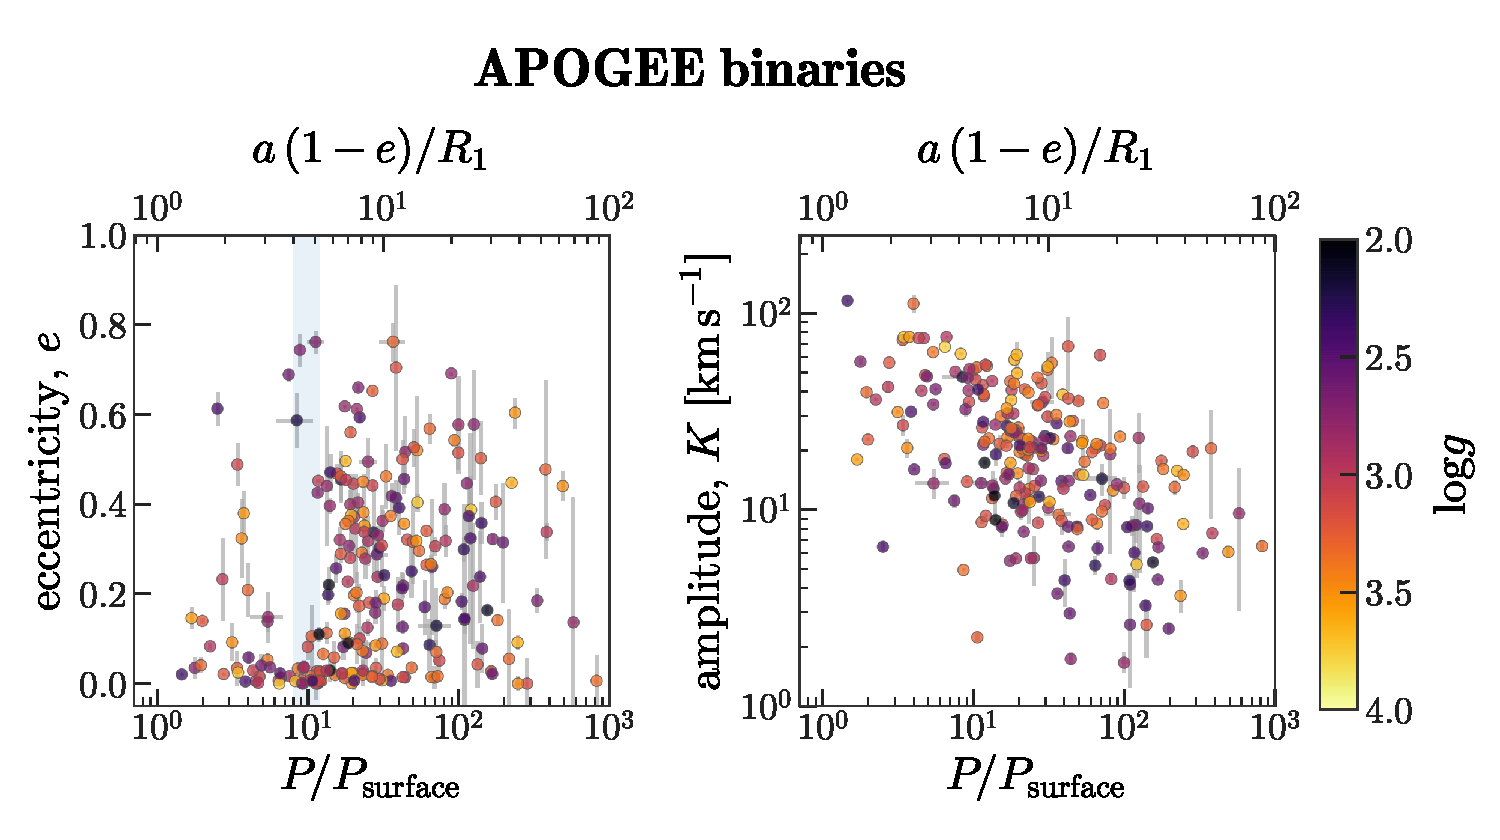
\includegraphics[width=\textwidth]{P-e-K}
\end{center}
\caption{%
\textit{Left panel:} Orbital period and eccentricity for all high-$K$ unimodal
systems with $\log g > 2$, with period values normalized by the orbital period
of a hypothetical companion at the surface of each primary star,
$P_{\textrm{surface}}$, assuming $M_1 = 1.36~\msun$ and $M_2 =0.5~\msun$.
Stars in the \apogee\ \DR\ red clump catalog are outlined in red.
The sharp transition from eccentric systems to almost all circular orbits at
$P/P_\textrm{surface} \approx 7$ is likely an outcome of tidal circularization.
\textit{Right panel:} Normalized period and inferred radial velocity amplitude
for the same systems.
Points below $P/P_\textrm{surface} = 1$ are likely systems where the primary and
companion mass assumptions used to compute $P_\textrm{surface}$ are invalid.
\label{fig:PeK}
}
\end{figure}


\section{Discussion}


\section{Conclusions}



\acknowledgements

It is a pleasure to thank ...

The authors are pleased to acknowledge that the work reported on in this
paper was substantially performed at the TIGRESS high performance computer
center at Princeton University which is jointly supported by the Princeton
Institute for Computational Science and Engineering and the Princeton
University Office of Information Technology's Research Computing department.

\software{
    \package{Astropy} (\citealt{Astropy-Collaboration:2013}),
    \package{emcee} (\citealt{Foreman-Mackey:2013}),
    \package{IPython} (\citealt{Perez:2007}),
    \package{matplotlib} (\citealt{Hunter:2007}),
    \package{numpy} (\citealt{Van-der-Walt:2011}),
    \package{scikit-learn} (\citealt{Pedregosa:2011}),
    \package{scipy} (\url{https://www.scipy.org/}),
    \package{schwimmbad} (\citealt{Price-Whelan:2017a}),
    \package{sqlalchemy} (\url{https://www.sqlalchemy.org/}),
    \package{thejoker} (\citealt{Price-Whelan:2017b}),
    \package{twobody} (\todo{twobody zenodo}).
}

\facility{\sdssiv, \apogee}

\clearpage

\bibliographystyle{aasjournal}
\bibliography{refs}


\end{document}
